\section{Experiments}
\label{sec:experiments}

We answer five research questions (RQs). \textbf{RQ1:} Without any annotations, can EoG improve LLM graph reasoning on different KGs? \textbf{RQ2:} Is each component of EoG necessary? \textbf{RQ3:} Can Graph Self-Play improve exploration through interaction? \textbf{RQ4:} Can SVTS replace human annotation as the training data source? \textbf{RQ5:} Can the curriculum advance from simple to complex topologies?

\subsection{Experimental Setup}

\textbf{Datasets.} We evaluate on WebQSP~\citep{webqsp}, CWQ~\citep{cwq}, and GrailQA~\citep{grailqa} over Freebase, GTSQA~\citep{GTSQA} and WikiWebQuestions~\citep{wikiwebquestions} over Wikidata, and IndustryCarBench, built on a real-world automotive-aesthetics KG of car models, design elements, colors, materials, and brands, with 500 expert-written test questions and no training set. Details of all six datasets are in Appendix~\ref{app:datasets}.

\textbf{Baselines.} We compare EoG with prompting-based (IO, CoT~\citep{CoT}, SC~\citep{Self-Consistency}), agent-based (ReAct~\citep{React}, ToG~\citep{ToG}, PoG~\citep{PoG}, CoR~\citep{CoR}), and retrieval-based methods (Text-Based Retrieval, Graph Reranker), all using the same backbone and KG as EoG. GraphWalker~\citep{GraphWalker} synthesizes data with closed-source models, which our setting excludes; the random-walk variant in Table~\ref{tab:ablation} approximates it. KG-R1$^\dagger$ (Section~\ref{sec:rq-svts}) is a fully supervised reference trained on the training set of each benchmark, whose annotations EoG never uses.

\textbf{Implementation Details.} Following prior work~\citep{ToG,KG-R1}, we report Hit@1 and F1. We build EoG on Qwen-2.5-3B/7B-Instruct~\citep{qwen25} and LLaMA-3.1-8B-Instruct~\citep{llama3}, and train it with Verl~\citep{sheng2025hybridflow} for 140 steps on 8 GH200 GPUs. The Solver uses GRPO and the Proposer REINFORCE, with 5 rollouts per task, a learning rate of $1\times10^{-6}$, and at most 15 assistant turns. Unless otherwise stated, analyses use Qwen-2.5-7B-Instruct on the three Freebase benchmarks. Appendix~\ref{app:training} lists the full set of hyperparameters.

\begin{figure*}[t]
\centering
\addtocounter{figure}{1}
\begin{minipage}[t]{0.245\linewidth}
  \centering
  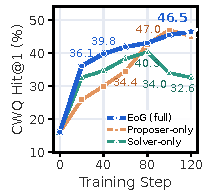
\includegraphics[width=\linewidth]{figures/RQ2_cwq_v2.pdf}\\[-2pt]
  {\small (a) CWQ Hit@1}
\end{minipage}\hfill
\begin{minipage}[t]{0.245\linewidth}
  \centering
  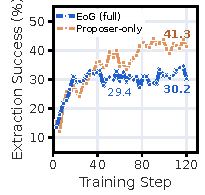
\includegraphics[width=\linewidth]{figures/RQ2_extraction_rate_v2.pdf}\\[-2pt]
  {\small (b) Extraction rate}
\end{minipage}\hfill
\begin{minipage}[t]{0.245\linewidth}
  \centering
  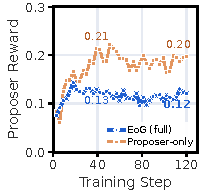
\includegraphics[width=\linewidth]{figures/RQ2_reward_proposer_v2.pdf}\\[-2pt]
  {\small (c) Proposer reward}
\end{minipage}\hfill
\begin{minipage}[t]{0.245\linewidth}
  \centering
  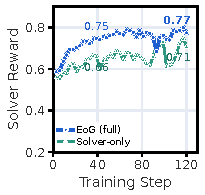
\includegraphics[width=\linewidth]{figures/RQ2_reward_solver_v2.pdf}\\[-2pt]
  {\small (d) Solver reward}
\end{minipage}
\caption{\textbf{Training dynamics of role ablations.} Proposer-only and Solver-only denote w/o Solver update and w/o Proposer update. (a) Validation Hit@1 on CWQ. (b) Question-extraction rate of the Proposer. (c--d) Proposer and Solver rewards.}
\label{fig:role_ablation}
\vspace{1mm}
\begin{minipage}[t]{0.48\textwidth}
  \vspace{0pt}
  \centering
  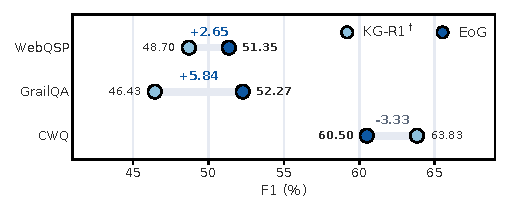
\includegraphics[width=\linewidth]{figures/RQ4_unseen_schema_f1.pdf}\par
  \refstepcounter{figure}
  \makeatletter
  \def\@currentlabelname{EoG vs. KG-R1 on unseen schema}
  \makeatother
  \label{fig:unseen_schema}
  \addcontentsline{lof}{figure}{\protect\numberline{\thefigure}{\textbf{EoG vs.\ KG-R1$^\dagger$ on unseen schema.} F1 (\%) of EoG and KG-R1$^\dagger$ trained on each dataset with Qwen-2.5-7B-Instruct.}}
  \noindent{\small\raggedright\textbf{Figure \thefigure: EoG vs.\ KG-R1$^\dagger$ on unseen schema. F1 (\%) of EoG and KG-R1$^\dagger$ trained on each dataset with Qwen-2.5-7B-Instruct.}\par}
\end{minipage}
\hfill
\begin{minipage}[t]{0.48\textwidth}
  \vspace{0pt}
  \centering
  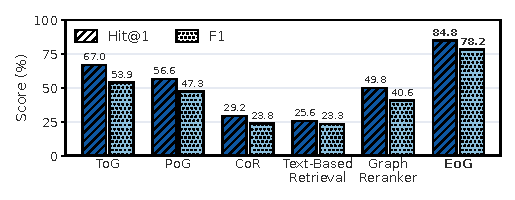
\includegraphics[width=\linewidth]{figures/RQ1_carbench_domain_v2.pdf}\par
  \addtocounter{figure}{-3}
  \refstepcounter{figure}
  \makeatletter
  \def\@currentlabelname{Results on IndustryCarBench}
  \makeatother
  \label{fig:carbench}
  \addcontentsline{lof}{figure}{\protect\numberline{\thefigure}{\textbf{Results on IndustryCarBench.} Hit@1 and F1 (\%) of EoG and baselines with Qwen-2.5-7B-Instruct.}}
  \noindent{\small\raggedright\textbf{Figure \thefigure: Results on IndustryCarBench. Hit@1 and F1 (\%) of EoG and baselines with Qwen-2.5-7B-Instruct.}\par}
  \addtocounter{figure}{2}
\end{minipage}

\end{figure*}


\subsection{Main Results (RQ1)}
\label{sec:main-results}
As shown in Table~\ref{tab:main_result} and Figure~\ref{fig:carbench}, without any question--answer annotations, EoG enables open-source LLMs to outperform prompting-, agent-, and retrieval-based methods on all three KGs. With Qwen-2.5-7B-Instruct, it exceeds the strongest baseline by \daulg{7.46} points in average Hit@1, and by \daulg{11.61} and \daulg{10.35} points on the multi-hop CWQ and GTSQA, showing that exploration learned through interaction handles complex questions better than retrieval or prompting. On Wikidata, EoG trains directly on the target KG and leads all annotation-free methods in Hit@1 on GTSQA and WikiWebQuestions, so the same pipeline carries over unchanged to a KG with a different schema. On IndustryCarBench, where annotation-based RL agents cannot be trained, EoG trains on the KG alone and exceeds the strongest baseline, ToG, by \daulg{17.80} points in Hit@1, so it applies directly to new KGs that lack annotations. On Qwen-2.5-3B and LLaMA-3.1-8B, against prompting baselines and ReAct, EoG leads in average Hit@1 and F1 (e.g., by 14.44 Hit@1 over SC on LLaMA-3.1-8B), and EoG on Qwen-2.5-3B (46.02) already surpasses PoG on Qwen-2.5-7B (45.54). On schema unseen in the annotations, EoG even outperforms the fully supervised KG-R1$^\dagger$ trained on WebQSP or GrailQA by 2.65 and 5.84 points in F1 (Figure~\ref{fig:unseen_schema}), showing that the exploration it learns through self-play over the whole KG generalizes well beyond the schema covered by annotations.

\subsection{Ablation Study (RQ2)}
\label{sec:ablation}
As shown in Table~\ref{tab:ablation}, we conduct an ablation study on Qwen-2.5-7B-Instruct-based EoG with five ablation settings: removing the Solver update; removing the Proposer update; replacing the query execution of SVTS with random walks~\citep{GraphWalker}, which walk backward from an answer entity and take the start entity as the only answer of the question; and replacing the Gaussian boundary reward with the adversarial reward $1-\bar{c}$ or the triangular boundary reward $1-2|\bar{c}-\frac{1}{2}|$, where $\bar{c}$ is the fraction of Solver trajectories that hit a gold answer. %
All five settings lower the Hit@1 on the multi-hop CWQ by 4.11--14.65 points, showing that Graph Self-Play, SVTS, and the curriculum each matter most on multi-hop questions.

\begin{figure*}[t]
\centering
\begin{minipage}{0.32\linewidth}\centering
  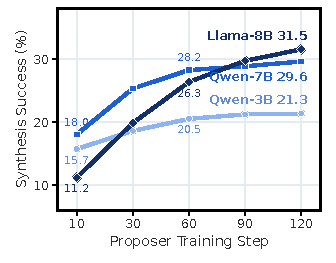
\includegraphics[width=\linewidth]{figures/RQ_4_synthesis_success_v2.pdf}\\{\small (a) Synthesis success}
\end{minipage}\hfill
\begin{minipage}{0.32\linewidth}\centering
  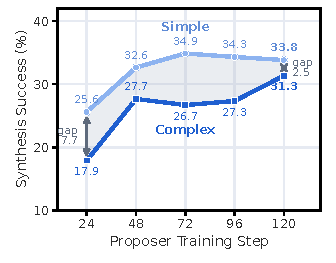
\includegraphics[width=\linewidth]{figures/RQ4_topology_easy_hard_v2.pdf}\\{\small (b) Simple vs.\ complex}
\end{minipage}\hfill
\begin{minipage}{0.32\linewidth}\centering
  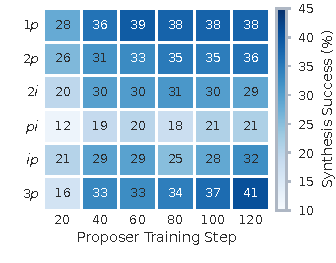
\includegraphics[width=\linewidth]{figures/RQ4_topology_success_heatmap_v2.pdf}\\{\small (c) Topology heatmap}
\end{minipage}
\caption{\textbf{Evolution of task difficulty.} Synthesis success rate of the Proposer over training steps (a) across three backbones, (b) on simple and complex topologies, and (c) per topology; complex topologies keep improving after simple ones plateau.}
\label{fig:frontier}
\vspace{-3mm}
\end{figure*}
\subsection{Analysis of Graph Self-Play (RQ3)}
\label{sec:rq-selfplay}

\textbf{Comparison with Training-Free Agents.} To examine whether exploration comes from interaction rather than the prompt, we compare EoG with its untrained starting point, ReAct. EoG improves the average Hit@1 of ReAct by more than 24 points on all three backbones and also surpasses ToG (Table~\ref{tab:main_result}), because the exploration strategy of a training-free agent cannot improve from interaction.
\begin{table}[t]
\caption{\textbf{Ablation study of EoG with Qwen-2.5-7B-Instruct on Freebase.} Bold marks the best result in each column.}
\label{tab:ablation}
    \centering
    \footnotesize
    \setlength{\tabcolsep}{2.4pt}
    \renewcommand{\arraystretch}{1.05}

    \begin{tabularx}{\columnwidth}{@{}l*{6}{>{\centering\arraybackslash}X}@{}}
    \toprule
    \multirow{2}{*}{\textbf{Variant}}
    & \multicolumn{2}{c}{\textbf{WebQSP}}
    & \multicolumn{2}{c}{\textbf{CWQ}}
    & \multicolumn{2}{c}{\textbf{GrailQA}}
    \\
    \cmidrule(lr){2-3}
    \cmidrule(lr){4-5}
    \cmidrule(lr){6-7}
    & \textbf{Hit@1} & \textbf{F1}
    & \textbf{Hit@1} & \textbf{F1}
    & \textbf{Hit@1} & \textbf{F1}
    \\
    \midrule
    \rowcolor{agentbg}
    ReAct (untrained)
    & 34.82 & 28.42 & 16.06 & 13.45 & 49.19 & 50.07 \\
    \midrule
    \rowcolor{ablrole}
    w/o Solver update
    & 53.74 & 47.08 & 46.39 & 42.15 & 58.50 & 55.69 \\
    \rowcolor{ablrole}
    w/o Proposer update
    & 63.14 & 56.91 & 36.22 & 35.83 & 55.67 & 55.18 \\
    \rowcolor{ablquery}
    w/o query exec. (Random Walk)
    & 64.87 & 57.67 & 35.93 & 35.64 & 60.12 & 60.41 \\
    \rowcolor{ablreward}
    Adversarial reward
    & 69.51 & 60.40 & 42.59 & 41.85 & 63.26 & 61.01 \\
    \rowcolor{ablreward}
    Triangular reward
    & \best{71.12} & \best{63.73} & 46.47 & 44.03 & 63.46 & 62.10 \\
    \midrule
    \rowcolor{lightblue}
    \textbf{EoG (full, Gaussian reward)}
    & 70.13 & 62.10 & \best{50.58} & \best{49.27} & \best{65.38} & \best{63.01} \\
    \bottomrule
    \end{tabularx}

\end{table}

\textbf{Impact of Removing the Solver Update.} We observe an interesting phenomenon: without Solver updates, the CWQ Hit@1 still rises from 16.06 to 46.39. We believe that proposing a question is itself a multi-hop graph exploration, which transfers to solving via the shared parameters. However, the variant still trails EoG by 16.39 and 6.88 on WebQSP and GrailQA, so the exploration gained from proposing only partly transfers; only when both roles are updated alternately do proposing and solving reinforce each other.

\subsection{Analysis of SVTS (RQ4)}
\label{sec:rq-svts}
To examine whether SVTS can replace human annotation, we design KG-R1$^\dagger$, a variant of KG-R1~\citep{KG-R1} that explores the full Freebase instead of a 2-hop subgraph pre-extracted for each question and differs from EoG only in being trained on annotated questions.

\textbf{Comparison with Human Annotation.} As shown in Table~\ref{tab:main_result}, KG-R1$^\dagger$ is stronger in distribution, but out of distribution, the annotation-free EoG achieves an average F1 3.05 and 3.65 higher than KG-R1$^\dagger$ trained on WebQSP and GrailQA, and trails KG-R1$^\dagger$ trained on 27,623 annotated CWQ questions by only 4.49. To examine generalization beyond the annotated schema, we split the Freebase test sets into seen and unseen schema by whether all relations in their SPARQL query appear in the training set of KG-R1$^\dagger$, and compare them on unseen schema (Figure~\ref{fig:unseen_schema}). EoG exceeds KG-R1$^\dagger$ trained on WebQSP and GrailQA by 2.65 and 5.84 in F1, although both lead on seen schema; KG-R1$^\dagger$ trained on CWQ still leads, but by 3.33 instead of 5.05. We believe that the gains of KG-R1$^\dagger$ from annotation are confined to the schema covered by its training set, whereas EoG trains on SVTS tasks sampled across the whole KG, so its graph reasoning transfers better to unseen schema.

\textbf{Comparison with Random-Walk Synthesis.} SVTS outperforms random walks on all three datasets, by 14.65 in Hit@1 on CWQ (Table~\ref{tab:ablation}), for two reasons. First, random walks favor chain paths and rarely yield the intersection or nested questions that multi-constraint reasoning needs. Second, a random walk takes only its start entity as the answer, although the same relations often reach several entities; correct Solver answers are then judged wrong, so the Proposer can hack the boundary reward with questions whose answers are not unique. SVTS instead executes the query to obtain the complete answer set, which removes such incorrect rewards. Moreover, the synthesized questions rarely resemble the test questions: only 2.28\% of them have a nearest Freebase test question with cosine similarity above 0.90 (Appendix~\ref{app:contamination}), so the gains of EoG do not come from test-set leakage into training.

\subsection{Analysis of the Boundary-Aware Graph Curriculum (RQ5)}
\label{sec:rq-frontier}

\textbf{Impact of Removing the Proposer Update.} Without Proposer updates, task topologies no longer follow the Solver: the Solver reward of this variant keeps rising, yet its CWQ Hit@1 drops after step 80 (Figure~\ref{fig:role_ablation}(a, d)), i.e., the Solver overfits the static task distribution of a Proposer without updates. This indicates that a Proposer without updates cannot shift to topologies that the Solver has not mastered, so the Solver stalls on early, simple questions and trails EoG by 14.36 points in Hit@1 on the multi-hop CWQ.

\textbf{Impact of the Boundary Reward.} We compare three Proposer rewards: the adversarial reward, the triangular boundary reward, and the Gaussian boundary reward. During training, the Solver occasionally produces overlong responses, which are truncated and temporarily lower its reward. With the adversarial reward, the Proposer cannot tell a hard question from such a truncated response and is rewarded most when the Solver performs worst: its reward drop lasts the longest among the three rewards, and its CWQ Hit@1 is 7.99 below that of the Gaussian boundary reward (Table~\ref{tab:ablation}). This shows that the Gaussian boundary reward is not reinforced by the Solver's truncated failures, so the curriculum returns to the Solver's capability boundary sooner after its outputs break down.

\textbf{Evolution of Task Difficulty.} As shown in Figure~\ref{fig:frontier}, the synthesis success rate of the Proposer rises on all three backbones (a), complex topologies rise from 17.9 to 31.3 while simple ones level off near 34, narrowing the gap to 2.5 points (b), and $3p$ keeps rising from 16 to 41 after simple patterns plateau (c), while the Solver reward does not decline (Figure~\ref{fig:role_ablation}(d)). This shows that the Proposer shifts toward complex topologies as the Solver improves, forming an adaptive graph curriculum that advances dynamically from easy to hard questions over time, without a manual schedule.

\subsection{Case Study}
\label{sec:case-study}
Appendix~\ref{app:case-study} shows one complete self-play round on a $2i$ task whose executed answer is Jersey. The Proposer finds that Jèrriais is spoken in Jersey, checks that French is also spoken there, and asks ``In which country are both Jèrriais and French spoken?'', which names both anchors but hides the answer. The Solver retrieves the countries of each language, among them Dominica, Mali, and Chad for French, and keeps only Jersey, the one country shared with Jèrriais. The Solver thus answers by intersecting two entity sets on the graph rather than recalling one fact, the reasoning that $2i$ tasks train.
